\chapter{\IfLanguageName{dutch}{Stand van zaken}{State of the art}}%
\label{ch:stand-van-zaken}

% Tip: Begin elk hoofdstuk met een paragraaf inleiding die beschrijft hoe
% dit hoofdstuk past binnen het geheel van de bachelorproef. Geef in het
% bijzonder aan wat de link is met het vorige en volgende hoofdstuk.

\paragraph{Inleiding}

\textbf{TODO:}
\\ 
achterliggende structuur webapplicatie uitleggen, Jhipster toevoegen en uitleg hiervan, SEO en ranking uitleggen, \textbf{note:} Leg ik best hier al gedetailleerder uit hoe de webscraping en antiwebscrapingstechnieken a.d.h.v gedetaillerdere voorbeelden of laat ik het zo met een gewone tekstuitleg en de voorbeelden pas aanhalen in mijn methodologie? Want ik wou dit dan ook doen aan de hand van de demoapplicatie maar hier is daar dan nog niets opgezet. Maar langs de andere kant is het nu vaak nog al onduidelijk/vaag uitgelegd is hoe technieken werken maar ga ik anders ook niet veel dubbel staan hebben in mijn methodologie? Weet niet zo goed wat te doen aangezien het zo wat dubbel is.

In dit hoofdstuk zal er meer informatie gegeven worden over wat web scraping is, hoe het werkt en wat de huidige maatregelen tegen web scraping zijn. 
\textbf{Note:} Zet ik hierin de litertuurstudie best ook extra informatie over hoe ik verwacht hoe de anti web scrapingstechnieken invloed zullen hebben op de performance? een voorbeeld hiervan is dat ik verwacht dat bij dynamische generatie, de pagina's veel trager gaan laden doordat er niet aan caching gedaan kan worden omdat de pagina altijd veranderd van structuur ==> geef ik hierbij dan meer info in de literatuurstudie over hoe de caching werkt?  
% Pas na deze inleidende paragraaf komt de eerste sectiehoofding.

\section{Terminologie}

\textbf{Note:}
\\ Hoort terminologie hier thuis? of moet dit eigenlijk in een andere sectie staan?

\subsection{HTTP protocol} \label{HTTP protocol}
Het Hypertext Transfer Protocol is een applicatie-level protocol dat gebruikt wordt bij distributed collaboratieve hypermedia informatiesystemen. Dit protocol dient om dataoverdracht te voorzien over het internet aan de hand van HTTP messages(zie \ref{HTTP message}) (\cite{rfc2616}). 
\subsection{HTTP message}\label{HTTP message}
Dit is de basiseenheid van HTTP communicatie en is opgebouwd uit de startlijn, header(-s)(zie \ref{Message header}), een lege lijn om het einde van de header(-s) aan te duiden en een eventuele message-body (\cite{rfc2616}).
\subsection{Message header} \label{Message header}
Een header wordt aanzien als een key-value pair om informatie mee te geven (\cite{rfc2616}).
\subsection{HTTP request} \label{HTTP request}
Een HTTP request message van een cliënt naar een server (\cite{rfc2616}).
\subsection{HTTP response} \label{HTTP response}
Een HTTP response message van een server naar een client nadat een request message geïnterpreteerd is (\cite{rfc2616}).
\subsection{Reguliere expressie} \label{Reguliere expressie}
Een reguliere expressies is een sequentie van karakters dat gebruikt wordt door de compiler als input. Vervolgens gaat de compiler een signaal geven elke keer als een string in de tekst overeenkomt met de reguliere expressie.  (\cite{10.1145/363347.363387})
\subsection{CSS Selectors} \label{css selectors}
CSS selectors zijn patronen die gebruikt worden om HTML elementen te selecteren gebaseerd op CSS properties zoals id, class, type, etc. (\cite{Persson2019}).


\section{Web scraping} \label{Web scraping}
In theorie is web scraping, ook bekend als web extraction of harvesten, de activiteit van het verzamelen van gegevens op een andere manier dan via API calls of menselijke interactie. Dit gebeurt meestal door het schrijven van een programma dat een website raadpleegt, gegevens opvraagt waaruit webpagina's bestaan, en die gegevens vervolgens verwerkt om er de benodigde informatie uit te halen en op te slagen in een bestand of database om deze vervolgens later op te vragen of te analyseren (\cite{Mitchell2018,Zhao2017}).
\\
\\
Web scraping is opgebouwd uit 3 verschillende fases, namelijk ophaling van data, extractie van data en transformatie van data. 
\begin{enumerate}
    \item \textbf{Ophaling van data}
\\
In deze fase moet de gewenste website bereikt worden aan de hand van het HTTP protocol (zie \ref{HTTP protocol}). De effectieve ophaling van data gebeurd  door een library die een HTTP GET request zal sturen naar een bepaalde URL en vervolgens de bijhorende webpagina terugkrijgt als een HTML document via de response ( \cite{Persson2019}).
    \item \textbf{Extractie van data}
\\
Bij deze fase wordt de data die gewenst is geëxtraheerd uit het HTML document verkregen in vorige fase. Dit gebeurd meestal aan de hand van REGEX, HTML parsing libraries of XPath queries om de gewenste data te vinden (\cite{Persson2019}).
    \item \textbf{Transformatie van data}
\\
Hierbij wordt de data die geëxtraheerd is getransformeerd in een gestructureerde versie (\cite{Persson2019}).
\end{enumerate}

\subsection{Web scraping methodes}
Niet alle web scraping libraries en frameworks benaderen de extractie van data op dezelfde manier. Zo bestaan er verschillende methoden om dit aan te pakken, zoals:
\begin{itemize}
    \item \textbf{Text Pattern Matching}
\\
Text pattern matching maakt gebruikt van reguliere expressies (zie \ref{Reguliere expressie}) om aan de hand van een patroon de gewenste tekst terug te vinden in het overkoepelend document. In deze paper gaat er niet verder worden ingegaan op text pattern matching aangezien de mogelijkheden van deze methode best beperkt zijn. (\textbf{Note} kan eventueel nog veranderen aangezien regex misschien als ondersteunende methode gebruikt gaat worden bij HTML parsing en dom parsing).
    \item \textbf{HTML Parsing a.d.h.v CSS selectors}
\\
Deze methode maakt gebruikt van de CSS selectors(zie \ref{css selectors}) om data te extraheren uit HTML documenten. Hierbij kan er gezocht worden op e.g. id's en klassen om de juiste data terug te vinden. (\cite{Persson2019})
\\
Om een voorbeeld te geven van hoe deze methode toegepast wordt, gaat er gebruik gemaakt worden van de HTML pagina gebaseerd op de code in figuur \ref{fig:figuur 1.1.png}. Stel nu dat de 3de heading de gewenste data omvat, kan er in dit geval HTML Parsing toegepast worden a.d.h.v de 'id' css selector. In dit specifiek geval zal vervolgens de tekst in '3de Heading' teruggeven worden.
\\

    \item \textbf{DOM Parsing}
In tegenstelling tot HTML parsing gaat DOM Parsing zich focussen op XPath (XML Path Language)  i.p.v css selectors. Xpath is een query taal dat gebruikt wordt om te navigeren in XML documenten en daarin eventueel selecties te maken. Xpath kan ook gebruikt worden om te navigeren in HTML documenten aangezien deze ook gebruik maken van de XML boomstructuur. (\cite{Persson2019,Mitchell2018})
\\
Om de werking van deze methode te tonen zal er weer gebruik gemaakt worden van de HTML pagina gebaseerd op de code in figuur \ref{fig:figuur 1.1.png}. Om het Xpath terug te vinden van de  3de heading voor DOM parsing moet er  gekeken worden naar de boomstructuur. In dit geval bevind deze header zich onder de <body> tag die zich vervolgens onder de <html> tag bevind. Afgeleid van deze informatie zal het Xpath van de 3de heading neerkomen op 
"/html/body/h1[3]". Dit resultaat kan vervolgens gebruikt worden om de tekst van de 3de Heading terug te geven.
    \item \textbf{Pagina analyse a.d.h.v computer visie en A.I}
Deze methode van web scraping kan vooral gebruikt in situaties waar de DOM obscuur is en vaak ge-update wordt maar de visuele structuur van de webpagina hetzelfde blijft. De gedachtegang voor deze methode is om een machine learning model te gaan trainen op gelabelde screenshots van een gelijkaardige website waarvan er wel makkelijk gescraped kan worden (e.g. webshop structuren zijn in het algemeen heel overeenkomend) of zelf een mock-up met mock-data op te zetten. Vervolgens wordt er a.d.h.v selenium aan screen capture gedaan van de gewenste te scrapen webpagina's en in real time geëvalueerd door het model en de gewenste data wordt uit deze foto's gehaald (bv. productnamen, product id's en prijzen bij een webshop). 
\\
\textbf{Note }van deze uitwerking heb ik geen effectieve goede bronnen van terug gevonden maar ik weet dat zulke services wel bestaan (https://www.diffbot.com/). Dit is eerder een gedachte van nog eventueel zelf uit te werken als ik hier de tijd voor heb maar leek me wel interessant om hier voorlopig bij te zetten en eventueel erna te verwijderen of effectief uit te werken. Maar aangezien ik hier geen bron van heb en dit mijn eigen gedachtengang is moet dit waarschijnlijk eerder bij de uitwerking?)
\end{itemize}

\begin{figure}[b]
    \centering
    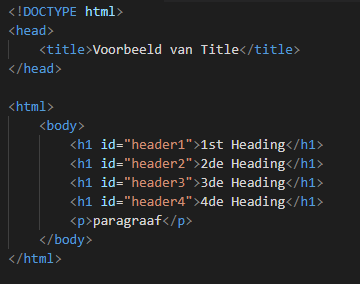
\includegraphics{bachproef/graphics/figuur 1.1.png}
    \caption{Voorbeeld van een simpele webpagina}
    \label{fig:figuur 1.1.png}
\end{figure}

\section{Anti web scraping methodes}
Zoals aangehaald in de paper \cite{10.1007/978-3-030-90016-8_4} is er een als maar stijgende vraag voor nieuwe en bruikbare data. Deze data wordt vaak niet manueel opgehaald maar hiervoor worden de vooraf aangehaalde methoden in sectie \ref{Web scraping} gebruikt, of specifieker de libraries en frameworks dat onderliggend gebruik maken van deze methoden. Om deze reden is het dan ook belangrijk om deze tegen te kunnen gaan. Zo bestaan er verschillende technieken om dit te bereiken, een paar voorbeelden aangehaald door \autocite{10.1007/978-3-030-90016-8_4} zijn:
\begin{itemize}
    \item \textbf{Rate limiting} 
    \\
Rate limiting werkt aan de hand van de snelheid van verzoeken op een website te beperken. Hierdoor kunnen web scraping programma's maar een bepaald aantal requests sturen naar de web server voordat ze buitengesloten worden.
    \item \textbf{Herkennen van automatisch netwerkverkeer} 
    \\
Deze techniek gaat zich eerder focussen naar het verwerken van informatie over het netwerkverkeer.
Dit is nu eenmaal mogelijk omdat web scrapers zich niet hetzelfde gedragen zoals humane gebruikers. 

Een paar indicatoren van web scrapers die gebruikt kunnen worden om hun buiten te sluiten zijn bijvoorbeeld:
\item Een hoog aantal paginabezoeken van hetzelfde ip-adres op een korte tijd
\item Een korte duratie van paginabezoeken aangezien web scrapers praktisch direct alle informatie verkrijgen van een webpagina en deze dan ook direct weer sluiten
\item  Netwerkverkeer uit landen dat onlogisch is. Lokale bedrijven gaan geen hoog aantal paginabezoeken krijgen uit landen aan de andere kant van de wereld. Dit duidt dan ook regelmatig op web scrapers. 
\item Een hoog aantal clicks op links die onlogisch lijken. Bv. leeg ingevulde contactformulieren, gebruikers die alle artikels in een webshop in hun winkelmandje plaatsen, etc.
\item Vreemde user-agents uitfilteren \textbf{Note: hier nog dieper op ingaan hoe user-agents werken, hoe ze er normaal moeten uitzien en hoe we vreemde user-agents kunnen vinden}
    
\item \textbf{Honey potting}
\\
Deze tactiek werkt door het strategisch plaatsen van  links of knoppen waardoor alleen bots ze kunnen vinden en gebruiken.
\textbf{}
\\
\\
Naast de voorbeelden uit de paper \cite{10.1007/978-3-030-90016-8_4} bestaan er nog verscheidene andere technieken die zullen uitgewerkt worden:
\item Dynamisch genereren van random id's en klassen. Door dit te randomiseren kan er geen gebruik gemaakt worden van bepaalde CSS selectors.
\item Dynamisch div's encapsuleren zodat de boomstructuur telkens veranderd. Op deze manier zal er ook geen mogelijkheid zijn om gebruik te maken van DOM parsing.
\item Tekst op de webpagina's tonen als foto.
\item Javascript gebruiken om de paginacontent te laden. Dit zorgt ervoor dat HTML parsers niet meer werken aangezien deze geen javascript runnen.
\end{itemize}



%Dit hoofdstuk bevat je literatuurstudie. De inhoud gaat verder op de inleiding, maar zal het onderwerp van de bachelorproef *diepgaand* uitspitten. De bedoeling is dat de lezer na lezing van dit hoofdstuk helemaal op de hoogte is van de huidige stand van zaken (state-of-the-art) in het onderzoeksdomein. Iemand die niet vertrouwd is met het onderwerp, weet nu voldoende om de rest van het verhaal te kunnen volgen, zonder dat die er nog andere informatie moet over opzoeken \autocite{Pollefliet2011}.

%Je verwijst bij elke bewering die je doet, vakterm die je introduceert, enz.\ naar je bronnen. In \LaTeX{} kan dat met het commando \texttt{$\backslash${textcite\{\}}} of \texttt{$\backslash${autocite\{\}}}. Als argument van het commando geef je de ``sleutel'' van een ``record'' in een bibliografische databank in het Bib\LaTeX{}-formaat (een tekstbestand). Als je expliciet naar de auteur verwijst in de zin, gebruik je \texttt{$\backslash${}textcite\{\}}.
%Soms wil je de auteur niet expliciet vernoemen, dan gebruik je \texttt{$\backslash${}autocite\{\}}. In de volgende paragraaf een voorbeeld van elk.

%\textcite{Knuth1998} schreef een van de standaardwerken over sorteer- en zoekalgoritmen. Experten zijn het erover eens dat cloud computing een interessante opportuniteit vormen, zowel voor gebruikers als voor dienstverleners op vlak van informatietechnologie~\autocite{Creeger2009}.

%\lipsum[7-20]
